\section{評価及び考察}
本システムの識別精度を確認するため,端末を持ち上げるモーションを対象とした実験を行った.
本システムを用いて6名の被験者にモーションを4回入力してもらい,データの収集を行った.
各被験者ごとに,最初の3回分を登録モードにおける学習データとして用い,最後の1回分を認証モードにおける入力データとして10回認証を試行した.
また,各試行時になりすまし認証データとして筆者自身が同様のモーションを行ったデータも入力した.
識別器より得られたデータを各被験者ごとに平均したものを表\ref{auth-result}に示す.
表中の数値が低いほど端末所有者のモーション入力であると意味しており,``本人''の列では数値が低いほど良く,``なりすまし''の列では数値が高いほど良い.

結果から,被験者EとFを除いて識別できているとわかる.
本システムでは,本人によるデータとなりすましによるデータを識別するためにダミーデータを用いた.
ダミーを含める割合は,増やしすぎるとなりすましによるデータから得られる識別器の出力が低くなり,減らしすぎると本人のデータから得られる識別器の出力が高くなるため,バランスを取る必要がある.
また,結果の良くなかった被験者EとFは終始データの変動が激しく,入力回数ごとで一致している部分があまり見られなかった.
これにより識別器の学習が進まず,上手く識別できなかったのではないかと考えられる.
識別率の良くなかった被験者Eのデータを図\ref{compare}に示す.

\begin{figure}[!tb]
  \def\@captype{table}
  \begin{minipage}{.48\textwidth}
    \centering
    \tblcaption{識別精度の評価結果}
    \label{auth-result}
    \begin{tabular}{|c|r|r|} \hline
      \multicolumn{1}{|c|}{}  & \multicolumn{1}{c|}{本人} & \multicolumn{1}{c|}{なりすまし} \\ \hline \hline
      A & 0.313607 & 0.999820 \\ \hline
      B & 0.472281 & 0.787281 \\ \hline
      C & 0.374718 & 0.539652 \\ \hline
      D & 0.453637 & 0.557697 \\ \hline
      E & 0.795578 & 0.642317 \\ \hline
      F & 0.458756 & 0.466918 \\ \hline
    \end{tabular}
  \end{minipage}
  %
  \hfill
  %
  \begin{minipage}{.48\textwidth}
    \centering
    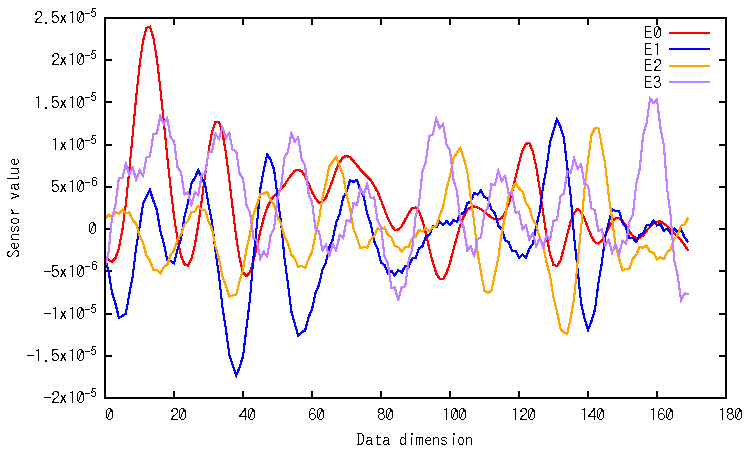
\includegraphics[bb=0 0 360 216, width=8cm]{Graphs/comp_E.pdf}
    \caption{被験者Eのデータ}
    \label{compare}
  \end{minipage}
\end{figure}
